\chapter{Mapeamento Sistemático da Literatura}
\label{cap:mapeamento}

Este capítulo relata o mapeamento sistemático conduzido para caracterizar o estado da arte na interseção entre gêmeos digitais urbanos, interoperabilidade semântica e sensibilidade ao contexto, e para fundamentar empiricamente a lacuna enunciada na Seção \ref{sec:problema}.

A escolha por uma busca sistemática decorre da natureza da afirmação que o trabalho precisa sustentar. Um único exemplo basta para afirmar que uma abordagem existe, mas afirmar que ela não existe exige ter procurado de modo exaustivo e declarado, sob pena de a ausência ser atribuída à busca e não ao campo. Como a contribuição aqui se apoia justamente em uma ausência, a de um artefato que reúna as cinco dimensões de comparação em um mesmo plano, a leitura dirigida não serve: ela encontra boas referências, mas não permite dizer o que não há. A opção pelo mapeamento, e não por uma revisão sistemática de eficácia, se justifica pelo caráter exploratório da questão: o objetivo é caracterizar a distribuição da pesquisa existente e localizar áreas com cobertura insuficiente, finalidade para a qual \citeonline{petersen2015guidelines} recomendam o instrumento, com as orientações operacionais de \citeonline{barn2017conducting} complementando a condução.

\section{Protocolo}
\label{sec:protocolo}

\subsection{Questões de mapeamento}

Os seis eixos de busca derivam das questões da Seção \ref{sec:questoes}, e essa correspondência permite atribuir cada resultado à pergunta que o motivou.

Da QP1, sobre o emprego de FIWARE e espaços de dados em gêmeos digitais urbanos, saiu o eixo de gêmeo digital urbano e arquitetura: expressões que cruzam o objeto com termos de arquitetura, \textit{middleware} e plataforma, somadas às que nomeiam o ecossistema e seus componentes de agregação. Da QP2, sobre mecanismos de contexto e raciocínio semântico, saíram dois eixos, o de sensibilidade ao contexto e o de interoperabilidade semântica e padronização, que vão do NGSI-LD e do \textit{context broker} aos modelos de dados e às normas de interoperabilidade. Da QP3, sobre a representação de perfis humanos, veio o eixo de centralidade humana e personalização, que reúne gêmeo digital humano, Sociedade 5.0 e perfilamento sensível ao contexto. Da QP4, sobre governança e proteção de dados, veio o eixo de espaços de dados e governança, que cobre conectores, soberania e os regimes de consentimento e privacidade.

Dois casos fogem dessa correspondência direta: o eixo de emergência e segurança pública, que não nasce de uma questão isolada, e a QP5, que não tem eixo próprio. O primeiro existe porque o cenário de referência do Capítulo \ref{cap:arquitetura} atravessa esse domínio, e serve à QP3 na parte de evacuação sensível a restrições individuais. A segunda é de outra natureza: pergunta o que falta na interseção dos eixos anteriores e só se responde depois de respondidas as quatro primeiras questões, tarefa da Seção \ref{sec:resultados-msl}.

\subsection{Critérios de inclusão e exclusão}
\label{sec:criterios}

Os critérios de inclusão (CI) e de exclusão (CE) da Tabela \ref{tab:criterios} foram combinados assim: incluiu-se o registro que satisfez CI5 e, simultaneamente, ao menos um entre CI1 e CI4, sendo os de exclusão eliminatórios. O recorte temporal de 2014 em diante corresponde à consolidação simultânea do ecossistema FIWARE e das primeiras formulações de gêmeo digital urbano; obras anteriores entraram apenas como fundamento conceitual, por inclusão dirigida, caso da formulação de contexto de \citeonline{dey2001understanding} e da sistematização do padrão \textit{Publish/Subscribe} de \citeonline{eugster2003many}.

\begin{table}[htb]
\centering
\caption{Critérios de inclusão e exclusão aplicados na triagem}
\label{tab:criterios}
\scriptsize
\begin{tabularx}{\textwidth}{@{}l X@{}}
\toprule
\textbf{Código} & \textbf{Critério} \\
\midrule
CI1 & Trata de arquitetura, plataforma ou \textit{middleware} para gêmeos digitais, cidades inteligentes ou espaços de dados. \\
CI2 & Aborda interoperabilidade semântica, gestão de contexto ou modelagem de dados urbanos. \\
CI3 & Reporta mecanismos de personalização, perfilamento ou centralidade no fator humano em ambientes urbanos ou industriais. \\
CI4 & Constitui especificação normativa, recomendação técnica ou \textit{position paper} de organismo de padronização relevante ao objeto. \\
CI5 & Publicado a partir de 2014, ou anterior mediante caráter fundacional reconhecido. \\
\midrule
CE1 & Não disponível em texto completo por meios institucionais. \\
CE2 & Redigido em idioma distinto de português, inglês ou espanhol. \\
CE3 & Emprega o termo \textit{digital twin} em domínio alheio ao urbano ou ao humano, sem contribuição arquitetural transponível. \\
CE4 & Constitui resumo expandido, editorial, prefácio ou material promocional. \\
CE5 & Duplicata de versão anteriormente incluída (preferiu-se a versão de periódico à de conferência). \\
\bottomrule
\end{tabularx}
\legend{Fonte: elaborada pelo autor.}
\end{table}

\subsection{Estratégia de busca}

A base primária é o Scopus, consultado por interface de programação com busca restrita ao campo \texttt{TITLE-ABS-KEY}, que compara a expressão contra título, resumo e palavras-chave do registro. Dois motivos sustentam a escolha: a cobertura e a busca restrita a campo. A cobertura contempla periódicos e anais de conferência publicados pelas organizações que concentram a produção do campo, entre elas IEEE, ACM, Springer, Elsevier e MDPI. A busca restrita a campo permite formular expressões booleanas verificáveis e recuperar todos os registros da base que as satisfazem, em lugar de uma amostra ordenada por relevância. Convém delimitar o alcance dessa afirmação: a recuperação é completa em relação à expressão, aos campos consultados e ao acervo indexado, o que não equivale a recuperar toda a literatura existente sobre o tema.

O OpenAlex entra como base complementar e cumpre três papéis, que convém separar porque não têm o mesmo peso. O primeiro é enriquecer os registros com palavras-chave, tópico e resumo, que a chave de acesso usada no Scopus não devolve. O segundo é recuperar pelo nome obras que a aferição da Seção \ref{sec:recobrimento} mostrou estarem fora da indexação do Scopus, caso de \citeonline{cirillo2019standard}, \citeonline{otto2019international} e \citeonline{komninos2016smart}. O terceiro é uma varredura temática por oito consultas, que devolveu 1.589 registros, 1.494 deles únicos dentro da própria base.

Essa terceira função pede uma ressalva. O OpenAlex não oferece busca restrita a campo nem permite percorrer o retorno inteiro de uma consulta: o teto é de 500 registros, e sete das oito consultas pararam em 200 de totais que somavam 74.757. O retorno da varredura é, portanto, uma amostra ordenada por relevância, exatamente o que a opção pelo Scopus procurou evitar. A diferença de regime fica declarada aqui e volta duas vezes adiante, na verificação da Seção \ref{sec:conducao} e entre as ameaças da Seção \ref{sec:ameacas-msl}. Quando este trabalho afirma recuperação exaustiva, a afirmação vale para a busca no Scopus.

As expressões foram construídas por faceta, cruzando o objeto com as dimensões do problema, e não por termo isolado. São 39 expressões distribuídas em seis eixos, resumidas na Tabela \ref{tab:expressoes}, todas qualificadas por \texttt{PUBYEAR > 2013}, que implementa o critério de janela temporal CI5 definido na Seção \ref{sec:criterios}. A paginação segue a ordenação cronológica por data de capa, que é o critério oferecido pela interface; como ela não declara desempate entre registros de mesma data, a garantia de recuperação integral não vem da ordenação, e sim da conferência entre o total que a base declara para cada expressão e o total efetivamente recebido, que coincidem nas 39.

A coluna \textit{Registros} da Tabela \ref{tab:expressoes} soma os retornos de cada expressão antes da deduplicação, de modo que um trabalho recuperado por três expressões é contado três vezes; o total de registros distintos consta da Tabela \ref{tab:triagem}. A coluna \textit{Removidas} traz as expressões redundantes de cada eixo, executadas mas não submetidas à triagem, pelo motivo discutido na Seção \ref{sec:conducao}. O texto integral das 39 expressões, com a justificativa de desenho de cada uma, está no repositório do projeto.

\begin{table}[htb]
\centering
\caption{Expressões de busca por eixo}
\label{tab:expressoes}
\scriptsize
\begin{tabularx}{\textwidth}{@{}X c r c@{}}
\toprule
\textbf{Eixo} & \textbf{Expressões} & \textbf{Registros} & \textbf{Removidas} \\
\midrule
Gêmeo digital urbano e arquitetura & 9 & 11.108 & -- \\
Interoperabilidade semântica e padronização & 9 & 3.883 & -- \\
Centralidade humana e personalização & 9 & 21.410 & 3 \\
Sensibilidade ao contexto & 4 & 3.258 & -- \\
Emergência e segurança pública & 5 & 12.175 & 2 \\
Espaços de dados e governança & 3 & 4.738 & 1 \\
\midrule
\textbf{Total} & \textbf{39} & \textbf{56.572} & \textbf{6} \\
\bottomrule
\end{tabularx}
\legend{Fonte: elaborada pelo autor.}
\end{table}

Como as expressões cobrem facetas adjacentes, um mesmo trabalho costuma aparecer em mais de uma, e o retorno das duas bases é reunido em uma única planilha antes de qualquer contagem. A deduplicação usa três chaves em escada: o identificador da base, o \textit{Digital Object Identifier} (DOI) normalizado e, por fim, o título normalizado com o ano. A escada existe porque nem todo registro traz DOI, caso de 4,4\% do conjunto que chegou à triagem; esses são deduplicados pelo identificador da base e, entre bases diferentes, pelo título. Os volumes resultantes aparecem na Seção \ref{sec:conducao}.

Antes da execução definitiva, as expressões passaram por um teste-piloto contra o conjunto de aferição descrito na Seção \ref{sec:recobrimento}, procedimento recomendado para calibrar a busca antes de confiar em seu retorno \cite{zhang2011identifying}. O piloto revelou dois defeitos de formulação, ambos corrigidos antes da coleta: o qualificador urbano, restrito a \texttt{urban} e \texttt{smart city}, não casava títulos ancorados em \textit{cities}, e foi ampliado em dez expressões; e nenhuma expressão alcançava revisões de estado da arte, porque todas exigiam uma faceta técnica, como o padrão semântico ou o componente de arquitetura, que uma revisão panorâmica não declara por tratar do campo inteiro. Daí a expressão de panorama. Os 56.572 registros relatados adiante provêm das 39 expressões já corrigidas, executadas por inteiro em uma única coleta.

{\setlength{\emergencystretch}{3em}%
A primeira ressalva de método quanto ao uso da interface é que a conjunção de um identificador com uma expressão de campo, na forma \texttt{DOI(x)} seguida de \texttt{AND TITLE-ABS-KEY(...)}, devolve zero resultados sempre que a expressão de campo começa por um grupo entre parênteses, mesmo quando o registro foi comprovadamente recuperado por aquela expressão submetida isoladamente. O comportamento foi verificado com quatro registros extraídos do próprio retorno de quatro expressões distintas, uma de cada eixo afetado: o identificador sozinho devolve um resultado e a conjunção devolve nenhum nos quatro casos. Por isso a aferição de recobrimento da Seção \ref{sec:conducao} foi conduzida por interseção entre o conjunto de identificadores do corpus de referência e o conjunto recuperado, e não por conjunção na própria consulta. A segunda ressalva é o teto de navegação da interface, que limita o deslocamento a 5.000 registros por consulta; nenhuma das 39 expressões o atinge, de modo que todas foram recuperadas por inteiro, sem necessidade de fatiamento por ano.\par}

\subsection{Procedimento de triagem}
\label{sec:procedimento-triagem}

Ler um a um os títulos recuperados não é viável no prazo desta pesquisa. A triagem por título e a atribuição de pertinência foram feitas, por isso, com apoio de um modelo de linguagem, que recebe um enunciado fixo e devolve uma decisão por registro. O enunciado é o texto de instrução entregue ao modelo: declara o objeto da pesquisa, reproduz os critérios de inclusão e exclusão da Seção \ref{sec:criterios} e fixa o formato da resposta. Ele é o mesmo para todos os registros, porque um enunciado que mudasse ao longo da triagem produziria decisões não comparáveis entre si. Assim, o classificador é o modelo operando sob aquele enunciado, e não o modelo isolado; a aferição incidiu sobre essa combinação.

A aferição confronta cada versão do enunciado com dois conjuntos de resposta conhecida. O primeiro reúne 49 obras pertinentes ao objeto, que são as do conjunto de aferição da Seção \ref{sec:recobrimento} que a busca alcançou; delas se extrai a \textit{sensibilidade}, a fração de obras pertinentes que a versão aprova, isto é, o quanto o classificador deixa de perder. O segundo reúne 49 registros de ruído inequívoco, retirados do que o filtro de domínio alheio havia descartado, como trabalhos que empregam \textit{digital twin} em manufatura ou em medicina; deles se extrai a \textit{especificidade}, a fração de ruído que a versão rejeita, isto é, o quanto o classificador deixa de desperdiçar.

As duas medidas puxam em sentidos opostos, e é esse o ponto da calibração. Um enunciado frouxo aprova quase tudo e não perde nada, ao custo de empurrar o ruído para a etapa seguinte; um enunciado rigoroso barra o ruído, mas começa a reprovar o que deveria passar. Cinco versões foram avaliadas, e a Figura \ref{fig:calibracao} mostra o resultado: cada ponto é uma versão do enunciado, e a linha pontilhada marca a sensibilidade mínima exigida para aceite. A segunda delas justifica todo o procedimento: uma exigência adicional que parecia inofensiva derrubou a sensibilidade para 0,73, ou seja, reprovou treze das obras que deveria ter aprovado. Sem a aferição prévia, essa perda teria passado despercebida.

\begin{figure}[H]
    \centering
    
    \begin{minipage}{0.70\textwidth}
        \caption{Calibração do classificador de triagem}
        \label{fig:calibracao}
        \centering

        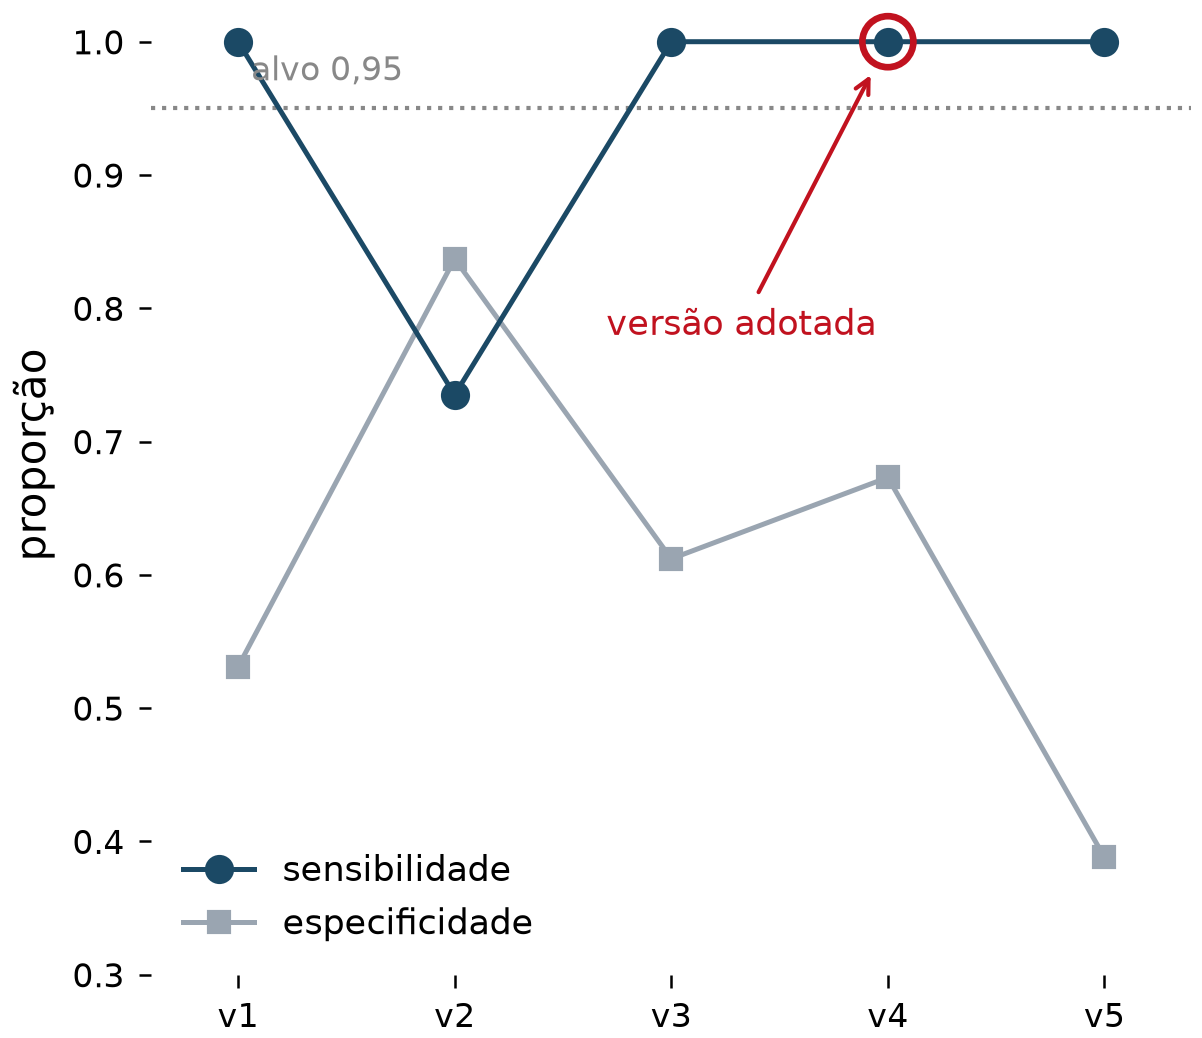
\includegraphics[width=0.80\linewidth]{Imagens/fig_calibracao.png}

        \par
        \raggedright
        \legend{Fonte: elaborada pelo autor.}
    \end{minipage}
\end{figure}

Adotou-se a quarta versão, que aprova as 49 obras e rejeita 67,3\% do ruído: entre as versões de sensibilidade 1,0, é a de maior especificidade. A assimetria é deliberada. Na triagem por título, excluir indevidamente é irreversível, porque o registro não volta a ser examinado, ao passo que incluir indevidamente custa apenas uma leitura a mais adiante.

Para efeito de reprodução, o classificador foi operado com o modelo Claude Opus, da Anthropic, em lotes de 250 registros, com saída estruturada e índice explícito por registro. Sem esse índice, o modelo perde a correspondência entre decisão e registro, defeito observado na aferição de custo. O enunciado adotado, as métricas das cinco versões e a decisão registrada para cada registro estão no repositório do projeto.

 

A triagem operou em dois passes. O primeiro decide apenas escopo, isto é, se o registro trata de algum dos eixos e guarda relação identificável com sistema de informação, dado ou especificação técnica. O segundo atribui grau de pertinência às questões de mapeamento, em quatro níveis: contribuição central, quando o artefato é o objeto declarado do trabalho; parcial, quando o aporte é secundário; tangencial; e não pertinente. Antes dos dois passes aplica-se um filtro determinístico de domínio alheio, que operacionaliza CE3 por marcadores léxicos inequívocos. Por ser determinístico, ele foi conferido contra o conjunto de aferição antes de valer: não derruba nenhuma das obras pertinentes. O volume que descarta consta da Seção \ref{sec:conducao}.

\subsection{Procedimento de extração}

De cada estudo incluído foram extraídos dois conjuntos de atributos, com funções metodológicas distintas. O primeiro é de caracterização e seleção: identificador persistente, metadados bibliográficos, questão de mapeamento principal e grau de pertinência. Esses atributos sustentam a caracterização do corpus da Seção \ref{sec:conducao} e definem, na Seção \ref{sec:relacionados}, quais estudos compõem a matriz comparativa. O segundo conjunto é de dimensões de comparação, codificadas apenas para os estudos admitidos na matriz. As dimensões são cinco: modelo semântico padronizado, barramento assíncrono exposto, perfil humano integrado ao contexto, governança e soberania instanciadas, e persistência segregada por natureza do dado. Cada uma recebeu uma entre três codificações: tratamento central e instanciado, quando a dimensão é objeto declarado da contribuição e o trabalho descreve mecanismo concreto que a realiza; tratamento parcial ou apenas declarativo; ou não abordado. Os símbolos correspondentes constam da Tabela \ref{tab:relacionados}. Essa codificação foi feita sobre o resumo de cada trabalho, recuperado pelo identificador persistente; nos casos em que o resumo não pôde ser obtido, a codificação apoiou-se em título, veículo e palavras-chave, e esses casos estão assinalados na própria tabela. Todos os passos, expressões e decisões foram registrados e estão disponíveis no repositório do projeto\footnote{\url{https://github.com/Alhexx/qualificacao}}, o que permite reexecutar o mapeamento de ponta a ponta.

\section{Condução e Caracterização do Corpus}
\label{sec:conducao}

As 39 expressões declararam 56.572 registros no Scopus e devolveram os mesmos 56.572, sem perda por teto de navegação em nenhuma delas. Somados os 1.589 registros do OpenAlex, chega-se a 58.161 registros brutos, que a Tabela \ref{tab:triagem} reduz por etapas.

Esses 58.161 são retornos, não trabalhos distintos: uma obra recuperada por três expressões aparece três vezes na contagem. A deduplicação resolve isso e remove 29,9\% do material, proporção que mede a sobreposição deliberada entre expressões vizinhas. Tomada cada base em separado, o Scopus responde por 39.646 registros distintos e o OpenAlex por 1.494, enquanto a união das duas produz 40.201. A soma das partes excede a união em 939, e essa diferença são os trabalhos que as duas bases recuperaram e que a união conta uma vez só; a contribuição exclusiva do OpenAlex fica, portanto, em 555 registros.

Sobre os 40.201 incidem os critérios eliminatórios. O filtro de tipo de documento descarta 1.656 registros por CE4, a janela temporal de CI5 descarta outros 26 e o filtro determinístico de domínio alheio retira 1.078. Restam 37.441 registros.

Antes da triagem, esse conjunto ainda perde o retorno de seis das 39 expressões de busca. Essas expressões foram executadas, mas, somadas, trazem cerca de treze mil registros que nenhuma outra expressão recupera, e entre eles há uma única obra do conjunto de controle. Deixá-las de fora reduz o conjunto de 37.441 para 24.314 registros e o recobrimento do conjunto de controle de 49 para 48 obras; os seis eixos continuam cobertos pelas expressões mais precisas de cada um.

O primeiro passe do classificador, a triagem por título, decide apenas se o registro está no escopo. Ele aprovou 17.985 dos 24.314 registros, sendo 15.267 por decisão de inclusão e 2.718 por dúvida, e reprovou 6.329. As 48 obras de controle presentes no conjunto foram todas aprovadas, o que confirma em escala real a sensibilidade medida na calibração sobre as 49 alcançadas pela busca.

O segundo passe atribui a cada um dos 17.985 aprovados um grau de pertinência às questões de mapeamento: contribuição central, parcial, tangencial ou não pertinente. Foram 1.942 registros de contribuição central e 5.345 de contribuição parcial, e o corpus incluído reúne esses dois graus, num total de 7.287 trabalhos. Os 10.698 restantes, tangenciais ou não pertinentes, ficam de fora. O ponto de corte, entre o grau parcial e o tangencial, foi fixado por medição: ele retém 44 das 48 obras de controle, e as quatro que ficam de fora são conceituais ou tangenciais, entre elas um levantamento de simulados de evacuação e uma discussão filosófica sobre centralidade humana em inteligência artificial \cite{taylor2023human}.

Por fim, resta saber quanto desse corpus depende da varredura temática no OpenAlex, que é a parte frágil do procedimento. Refazendo a contagem só com o que veio do Scopus, o corpus incluído passa de 7.287 para 6.887 trabalhos, e os de contribuição central, de 1.942 para 1.775. A base complementar responde por 5,5\% do corpus e por 8,6\% do seu núcleo, e o padrão descrito na Seção \ref{sec:relacionados} se sustenta sobre os 1.775 do Scopus como se sustentava sobre os 1.942. Pode-se afirmar, portanto, que o impacto da varredura sobre o resultado é baixo.

\begin{table}[htb]
\centering
\caption{Etapas de triagem e volumes resultantes}
\label{tab:triagem}
\scriptsize
\begin{tabularx}{\textwidth}{@{}X r@{}}
\toprule
\textbf{Etapa} & \textbf{Registros} \\
\midrule
Expressões de busca submetidas ao Scopus & 39 \\
Registros declarados pela base & 56.572 \\
Registros recuperados no Scopus & 56.572 \\
Registros recuperados no OpenAlex & 1.589 \\
\midrule
Total bruto & 58.161 \\
Únicos após deduplicação por identificador, DOI e título & 40.201 \\
Após filtro de tipo de documento (CE4) & 38.545 \\
Após janela temporal (CI5) & 38.519 \\
Após filtro determinístico de domínio alheio (CE3) & 37.441 \\
\midrule
Submetidos à triagem por título & 24.314 \\
Aprovados quanto ao escopo & 17.985 \\
Classificados como de contribuição parcial & 5.345 \\
Classificados como de contribuição central & 1.942 \\
\midrule
\textbf{Corpus incluído} & \textbf{7.287} \\
Conjunto comparativo após S1 e S2 & 822 \\
\bottomrule
\end{tabularx}
\legend{Fonte: elaborada pelo autor.}
\end{table}

\subsection{Recobrimento aferido}
\label{sec:recobrimento}

Uma busca automatizada só sustenta uma afirmação de ausência se tiver sido aferida. A aferição aqui segue a prática de confrontar a busca com um conjunto de obras pertinentes reunido por outro caminho, que \citeonline{zhang2011identifying} denominam \textit{quasi-gold standard}: obras identificadas antes da busca, por leitura do domínio e encadeamento de referências ao longo da pesquisa exploratória.

A composição desse conjunto obedece a uma regra declarada, e não à preferência do pesquisador. Entram as obras cujo objeto declarado pertence ao escopo do mapeamento, isto é, gêmeo digital urbano, plataforma de cidade inteligente, contexto e semântica urbana, perfil humano ou resposta a emergência, desde que indexadas com identificador persistente e dentro da janela temporal. Ficam de fora a fundamentação de engenharia de software transversal, sobre mensageria, conteinerização, microsserviços e bancos de série temporal, e os guias de condução de mapeamento sistemático \cite{petersen2015guidelines,barn2017conducting}. Essas obras não tratam do objeto do mapeamento, e uma busca bem delimitada não deve encontrá-las. Se entrassem na aferição, cada uma contaria como falha da busca, quando a ausência delas é justamente o resultado esperado. Elas entram no trabalho por inclusão dirigida declarada, mecanismo previsto no protocolo e recomendado por \citeonline{petersen2015guidelines}.

Das 78 obras reunidas, a regra mantém 64 na aferição, e a busca alcança 49 delas, um recobrimento de 76,6\%. As quinze restantes se explicam por quatro motivos: a falta do qualificador urbano, o domínio adjacente, a indexação irregular e o filtro de tipo de documento. Cinco são obras gerais, entre elas a formulação original do conceito de gêmeo digital \cite{grieves2016digital}, as revisões de maior circulação do campo \cite{barricelli2019survey,rasheed2020digital,vanderhorn2021digital} e um levantamento de \textit{middleware} sensível ao contexto social \cite{liang2015social}. Nenhuma expressão as alcança porque todas exigem o qualificador urbano, que é decisão deliberada do recorte, e por isso são ausências por construção, não por falha. Quatro estão em veículos de domínio adjacente, como pesquisa operacional, planejamento urbano, mobilidade e marketing, cujo vocabulário não cruza as facetas técnicas das expressões. Cinco estão fora da indexação regular do Scopus: três capítulos de livro ou periódicos de indexação irregular e duas obras apresentadas em conferências brasileiras. A última, uma nota editorial sobre a passagem da cidade inteligente ao gêmeo digital urbano \cite{yeh2024from}, foi alcançada pela busca e descartada pelo filtro de tipo de documento.

Por trás dessa leitura está uma distinção que convém deixar explícita: o corpus do mapeamento não coincide com a bibliografia deste trabalho. O mapeamento recupera o estado da arte do objeto, ao passo que a fundamentação tecnológica e metodológica chega por inclusão dirigida. Um protocolo que recuperasse por expressão temática um estudo comparativo de bancos de série temporal estaria mal delimitado, e não melhor calibrado.

A Figura \ref{fig:corpus} caracteriza os 7.287 trabalhos incluídos. A distribuição temporal mostra crescimento acelerado e recente, com mais da metade do corpus publicada de 2024 em diante, o que mostra um campo ainda em consolidação. A distribuição por questão de mapeamento concentra 3.009 trabalhos em QP1, contra 1.031 em QP3 e 1.018 em QP4, assimetria que mostra o campo concentrado na infraestrutura de interoperabilidade, e não em integrar o fator humano ou em instanciar governança. A assimetria, por si só, não estabelece a lacuna, uma vez que mil trabalhos em QP3 atestam a existência de pesquisa sobre o tema; o que ela indica é que o esforço se reparte entre frentes que raramente se encontram no mesmo artefato, observação que a matriz da Seção \ref{sec:relacionados} qualifica no nível do trabalho individual.

\begin{figure}[H]
	\centering
	\caption{Caracterização do corpus incluído}
	\label{fig:corpus}
	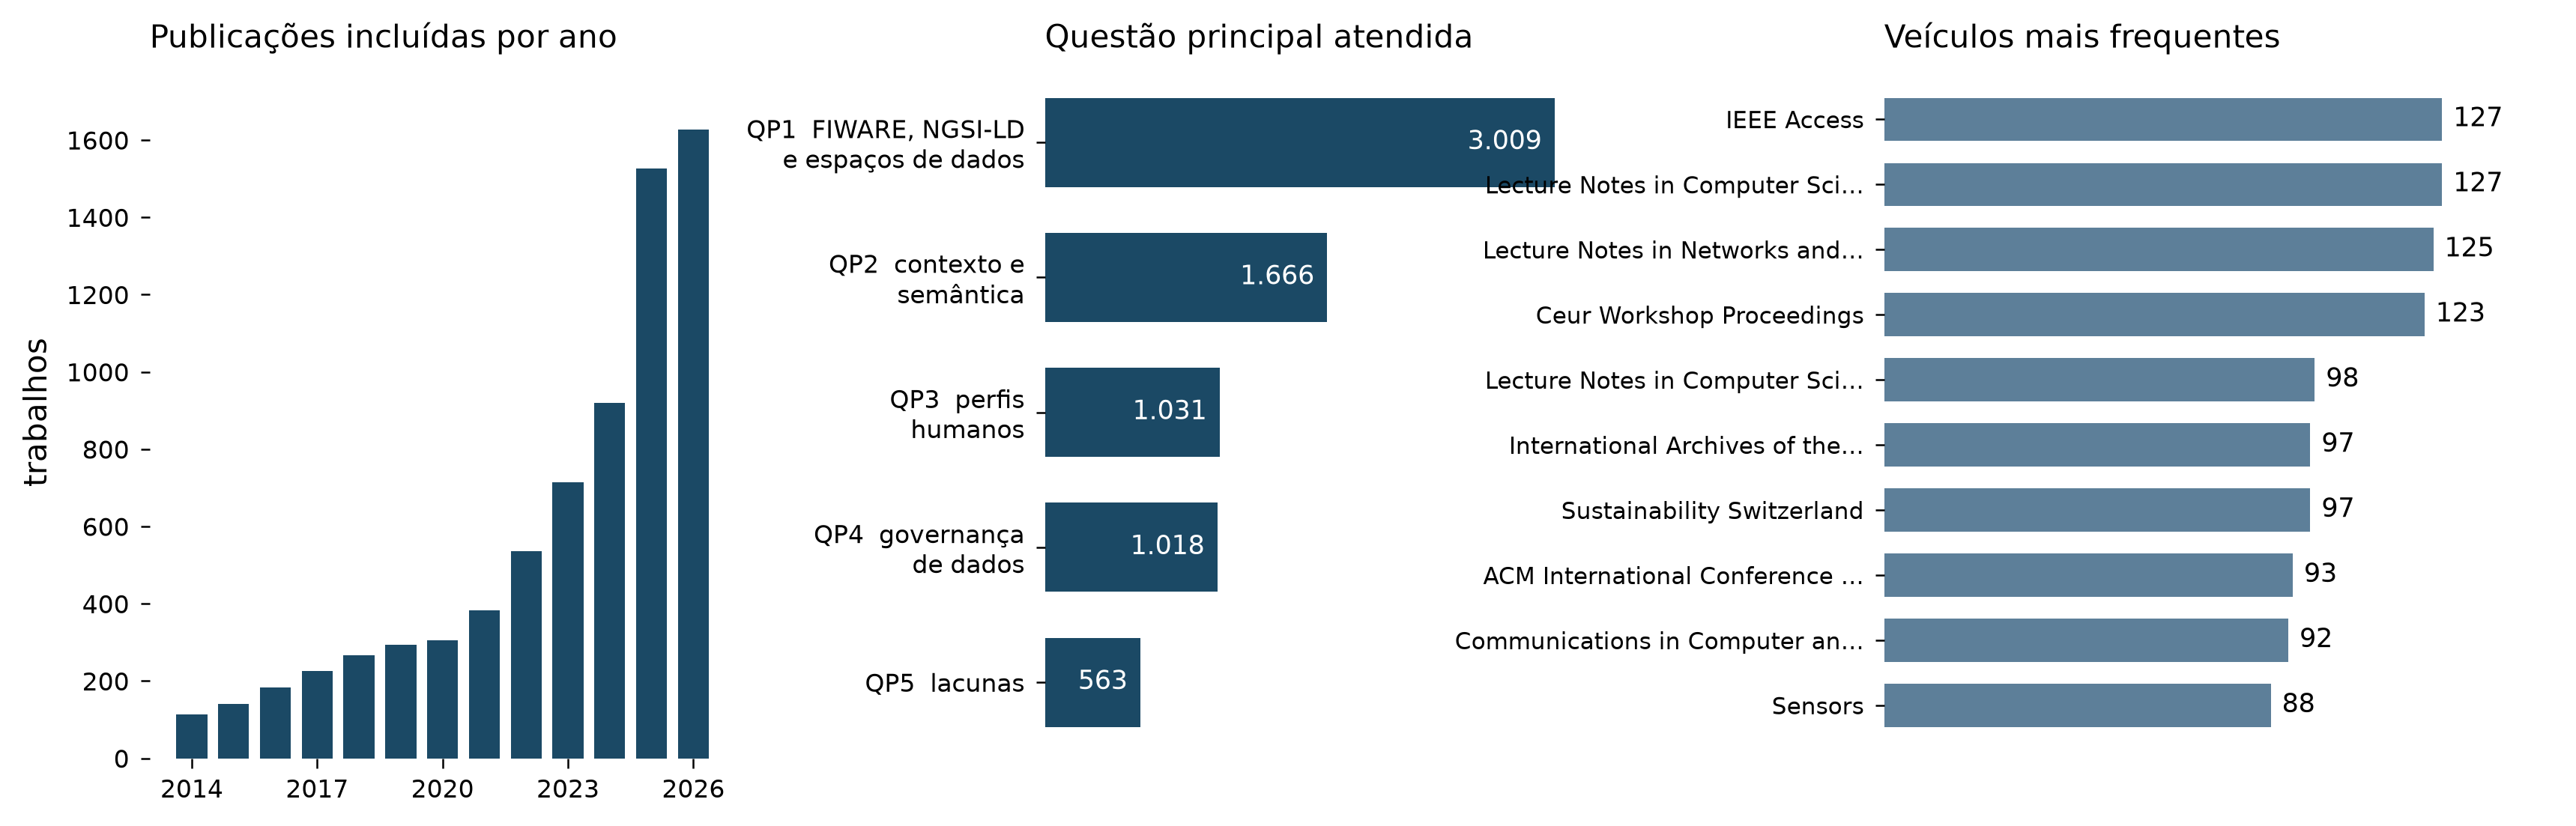
\includegraphics[width=\textwidth]{Imagens/fig_corpus.png}
	\legend{Fonte: elaborada pelo autor sobre os 7.287 trabalhos incluídos. A questão de mapeamento principal é atribuída na triagem de pertinência, descrita na Seção \ref{sec:procedimento-triagem}.}
\end{figure}

\section{Resultados por Questão de Mapeamento}
\label{sec:resultados-msl}

A QP1 pergunta como o FIWARE e os espaços de dados têm sido empregados na construção de gêmeos digitais urbanos e quais componentes se repetem nessas soluções. Para o FIWARE, a resposta é clara: o corpus o confirma como ecossistema de referência para plataformas urbanas abertas. Quando ele é levado a gêmeos digitais urbanos, como em \citeonline{bauer2021urban} e \citeonline{ditorrepadula2025smart} \cite{cirillo2019standard,bauer2022fiware,salhofer2019building}, repete-se o mesmo arranjo: o \textit{Context Broker}, uma camada de conexão a dispositivos e uma camada de persistência histórica. A ele se associam identidade e autorização. Somam-se a esses trabalhos plataformas municipais em operação. Entre elas estão o concentrador coreano de dados urbanos construído sobre padrões abertos \cite{jeong2020city} e a arquitetura de cidade baseada em conhecimento de \citeonline{badii2017analysis}. Na mesma linha, o arcabouço DUET interliga gêmeos digitais urbanos interoperáveis em escala europeia \cite{raes2022duet}. Nesse conjunto, o barramento de mensageria continua aparecendo como detalhe interno do broker, sem ser exposto como ponto de extensão, isto é, como lugar em que outros serviços possam se conectar ao fluxo de mudanças.

Para os espaços de dados, a resposta é menos coesa. A literatura se divide em duas frentes que pouco dialogam: uma trata dos modelos de referência e dos arranjos de governança, e a outra propõe a convergência entre espaços de dados e gêmeos digitais \cite{otto2019international,idsa2022ram,tardieu2022role,gaiax2022architecture,somma2023digital,uslander2022symbiotic,coppolino2025simulation,vogt2024towards}. No plano urbano, \citeonline{cuno2019data} são a referência mais direta. O trabalho de \citeonline{galij2025evaluating} é o único do corpus a quantificar a sobrecarga de desempenho da camada de soberania, e esse achado entrou como restrição de projeto na Seção \ref{sec:governanca}.

A QP2 pergunta que mecanismos de sensibilidade ao contexto e de raciocínio semântico as arquiteturas de gêmeos digitais urbanos reportam, e a resposta é a mais fragmentada. A literatura de \textit{middleware} sensível ao contexto é tecnicamente sofisticada \cite{lopes2009context,lopes2013middleware,liang2015social,sezer2018context}, mas antecede a consolidação do NGSI-LD e não dialoga com o vocabulário de gêmeos digitais. Já os trabalhos de gêmeos urbanos que discutem raciocínio tratam de simulação física, e não de raciocínio simbólico sobre os relacionamentos entre entidades. Os que mais se aproximam investigam como representar o NGSI-LD em RDF e consultá-lo em \textit{SPARQL Protocol and RDF Query Language} (SPARQL), as linguagens da Web Semântica para descrever e consultar grafos \cite{abid2022toward,viola2019mapping,drobnic2026automatic,gonzalez2024reshaping}. Eles demonstram que é viável percorrer o grafo de relacionamentos, mas tratam essa travessia como problema de consulta e não prescrevem como ligar o resultado a um fluxo que reage a eventos em tempo crítico. \citeonline{gao2017automated} descrevem a descoberta e a composição automatizadas de fluxos sobre dados urbanos semânticos, e \citeonline{bouloukakis2023enabling} constroem sobre NGSI uma camada de publicação e assinatura para sistemas de transporte. Os dois estreitam a distância entre raciocínio e resposta reativa, mas ficam no nível de um componente isolado, sem trazer perfil humano nem governança para o mesmo desenho. Em outra direção, \citeonline{austin2020architecting} combinam modelo semântico e aprendizado de máquina numa arquitetura de gêmeo digital urbano, e \citeonline{an2019global} propõem um adaptador semântico para a interoperação entre cidades.

A QP3 pergunta como os perfis humanos, com suas restrições de acessibilidade e vulnerabilidades, são representados e integrados ao modelo de contexto urbano. No domínio industrial, essa representação está madura \cite{asad2023human,okegbile2022edge}. No urbano, ainda é incipiente. O cidadão aparece como fonte de percepção e de participação \cite{luo2025perception,qanazi2025integrating}. A literatura também analisa de forma crítica a agência cidadã, isto é, o quanto ele de fato age sobre os sistemas que o envolvem \cite{tappert2024citizen,dejaeger2026right}. Só a literatura de evacuação e mobilidade trata restrição de acessibilidade como atributo que o sistema usa em cálculo \cite{hashemi2018emergency,deng2022semantic,allahbakhshi2026zuriact,wins2024enhancing}. Cada trabalho dessa linha, porém, usa um modelo de perfil próprio, sem integração a um modelo de contexto urbano padronizado. O precedente mais próximo está em \citeonline{liu2023urban}, que montam perfis de usuários móveis sobre um grafo de conhecimento urbano, embora para recomendar conteúdo e não para responder a emergências. \citeonline{zeng2025knowledge} oferecem um precedente de natureza análoga, combinando grafo de conhecimento e modelo oculto de Markov para personalização urbana, e \citeonline{rivadeneira2024confluence} propõem um modelo de integração que põe o humano no laço de decisão. Nenhum estudo do corpus, porém, representa o perfil humano como entidade NGSI-LD de primeira classe, ligada por relacionamentos às edificações e aos eventos no mesmo grafo.

A QP4 pergunta que estratégias de governança, soberania e proteção de dados as plataformas urbanas federadas adotam quando atributos pessoais sensíveis entram no processamento. A literatura concentra-se em três mecanismos: o conector como ponto único de aplicação de política, a identidade auto-soberana e a arquitetura corporativa de referência para efetivar a soberania digital \cite{idsa2022ram,gaiax2022architecture,sanchezserna2026data,firdausy2022towards}. Na identidade auto-soberana, o titular controla as próprias credenciais, sem depender de um provedor central. Soma-se a eles a identificação de vetores de exposição de perímetro, os pontos por onde um ataque pode atravessar a fronteira da plataforma \cite{perata2023security}. A literatura de gêmeos digitais urbanos, porém, raramente instancia esses mecanismos, e na maioria dos trabalhos a privacidade continua no plano das declarações de princípio. A análise de riscos de \citeonline{fontes2024human} é a exceção mais consistente. A ontologia de consentimento e contrato de \citeonline{kurteva2023smashhitcore} vai além, porque modela em vocabulário formal os elementos que a proteção de dados pessoais exige em dados de sensores. É o precedente mais próximo do tratamento de consentimento que a Seção \ref{sec:governanca} adota.

A QP5 pergunta que lacunas permanecem abertas na interseção dos eixos anteriores. A resposta sai das quatro questões anteriores, na forma de cinco lacunas que a Seção \ref{sec:requisitos} liga aos requisitos:

\begin{description}[leftmargin=1.6cm,style=nextline]
	\item[L1] Perfil humano fora do grafo de contexto. Quando existem, os perfis ficam em bases separadas do modelo de contexto urbano, e por isso não é possível partir de um evento, passar pela infraestrutura e chegar à pessoa afetada percorrendo relacionamentos.
	\item[L2] Barramento de eventos tratado como detalhe interno. O fluxo de mudanças de contexto raramente é exposto para que outros serviços o assinem, o que obriga integrações por consulta periódica e eleva a latência de resposta.
	\item[L3] Dissociação entre raciocínio semântico e ciclo reativo. Percorrer relacionamentos é tratado como problema de consulta, e não como etapa do fluxo assíncrono que decide a resposta em tempo crítico.
	\item[L4] Governança declarativa, não instanciada. Os mecanismos de soberania aparecem como requisito, mas raramente viram componentes arquiteturais auditáveis, e seu custo de desempenho quase nunca é medido.
	\item[L5] Persistência única para dois perfis de acesso. Consultas geoespaciais sobre o estado corrente e agregações sobre séries históricas convivem nos mesmos mecanismos de persistência, e raramente motivam separá-los de forma deliberada.
\end{description}

\section{Trabalhos Relacionados}
\label{sec:relacionados}

Comparar trabalhos lado a lado exige decidir antes quais entram na comparação, e essa decisão precisa de regra explícita, sob pena de a matriz refletir a composição da amostra em lugar do estado do campo. A regra parte dos 1.942 trabalhos de contribuição central e faz duas perguntas, nas quais o trabalho precisa passar. A primeira, S1 (escala da contribuição), é se ele propõe algo que se possa posicionar na matriz. Valem arquitetura, plataforma ou sistema completo, especificação normativa de arquitetura e componente que instancie tecnicamente ao menos uma das cinco dimensões de comparação. Revisões e estudos puramente empíricos ficam de fora, por não proporem artefato. A segunda, S2 (ancoragem urbana), é se o objeto declarado do trabalho é a cidade, a infraestrutura urbana ou os serviços públicos urbanos. Nenhuma das duas perguntas olha para as dimensões da matriz: S1 e S2 decidem quem entra pela escala e pelo domínio, e as dimensões decidem o que se observa em cada trabalho admitido. Essa independência faz a matriz produzir evidência, e não repetir o próprio critério de entrada.

As duas perguntas retêm 822 trabalhos, conjunto grande demais para leitura integral. A Tabela \ref{tab:relacionados} confronta 15 deles, também escolhidos por regra declarada. Entram todos os que tratam duas dimensões como centrais e todos os que tratam como central alguma das quatro dimensões menos estudadas: comunicação assíncrona, perfil humano, governança e persistência segregada. As vagas restantes vão aos de maior pontuação somada nas cinco colunas, com dois pontos por tratamento central e um por parcial. A codificação apoia-se no resumo de cada trabalho, recuperado pelo identificador persistente, e o único caso em que o resumo não pôde ser obtido está assinalado na tabela.

\begin{table}[htb]
\centering
\caption{Posicionamento comparativo dos trabalhos relacionados}
\label{tab:relacionados}
\scriptsize
\begin{tabular}{@{}p{4.1cm}p{4.6cm}ccccc@{}}
\toprule
\textbf{Trabalho} & \textbf{Foco principal} & \hdrv{Modelo\\semântico} & \hdrv{Barramento\\assíncrono} & \hdrv{Perfil\\humano} & \hdrv{Governança} & \hdrv{Persistência\\segregada} \\
\midrule
\citeonline{badii2017analysis} & Arquitetura de cidade baseada em conhecimento com APIs de serviço & $\bullet$ & $\circ$ & -- & $\circ$ & $\circ$ \\
\citeonline{gao2017automated} & Middleware de descoberta e composição semântica de fluxos urbanos & $\bullet$ & $\bullet$ & $\circ$ & -- & -- \\
\citeonline{cheng2018fogflow} & Arcabouço de computação em névoa para serviços IoT urbanos & $\circ$ & $\bullet$ & -- & -- & -- \\
\citeonline{souza2018geographic} & Middleware de camadas geográficas para dados urbanos & $\circ$ & -- & -- & -- & $\bullet$ \\
\citeonline{cuno2019data} & Espaço de dados urbanos para soberania sobre arquiteturas de referência & $\circ$ & -- & -- & $\bullet$ & -- \\
\citeonline{jeong2020city} & Plataforma coreana de dados urbanos baseada em modelo comum & $\bullet$ & $\circ$ & -- & $\circ$ & -- \\
\citeonline{bauer2021urban} & Gêmeo digital urbano baseado em FIWARE e NGSI-LD & $\bullet$ & $\circ$ & -- & -- & -- \\
\citeonline{pereira2022platform}\,$^{\dagger}$ & Plataforma de integração de dados heterogêneos para aplicações urbanas & $\circ$ & -- & -- & $\circ$ & $\circ$ \\
\citeonline{raes2022duet} & Arcabouço DUET de gêmeos digitais urbanos interoperáveis e confiáveis & $\circ$ & $\circ$ & $\circ$ & $\circ$ & -- \\
\citeonline{bouloukakis2023enabling} & Plataforma NGSI publish/subscribe para transporte público IoT & $\bullet$ & $\bullet$ & -- & -- & -- \\
\citeonline{kurteva2023smashhitcore} & Ontologia de consentimento e contratos para conformidade com GDPR & $\bullet$ & -- & $\circ$ & $\bullet$ & -- \\
\citeonline{liu2023urban} & Grafo de conhecimento urbano para perfilamento de usuários móveis & $\bullet$ & -- & $\bullet$ & -- & -- \\
\citeonline{gonzalez2024reshaping} & Enriquecimento semântico de dados urbanos com NGSI-LD & $\bullet$ & $\circ$ & $\circ$ & -- & -- \\
\citeonline{rivadeneira2024confluence} & Modelo de integração IoT com humano no laço e privacidade preservada & $\circ$ & -- & $\circ$ & $\bullet$ & -- \\
\citeonline{zeng2025knowledge} & Grafo de conhecimento e modelo oculto de Markov para rotas personalizadas & $\bullet$ & -- & $\bullet$ & -- & -- \\
\midrule
\textbf{Proposta desta pesquisa} & Backend sensível ao contexto para gêmeo digital urbano & $\bullet$ & $\bullet$ & $\bullet$ & $\bullet$ & $\bullet$ \\
\bottomrule
\end{tabular}
\par\vspace{4pt}
\legend{Fonte: elaborada pelo autor. $\bullet$ tratamento central; $\circ$ tratamento parcial; -- não abordado. $^{\dagger}$ codificação apoiada em título, veículo e palavras-chave, por indisponibilidade do resumo.}
\end{table}

A coluna de semântica é a mais ocupada: entre os 15, são 9 tratamentos centrais e 6 parciais, e nenhum trabalho a ignora por completo. Isso reflete a maturidade que as plataformas urbanas abertas já consolidaram nesse eixo. As outras quatro colunas estão bem mais vazias. Comunicação assíncrona registra 3 tratamentos centrais, governança 3, perfil humano 2 e persistência segregada apenas 1, contra 12 trabalhos que não a abordam.

Nenhum dos 15 trabalhos trata como central mais de duas das cinco dimensões, e cinco chegam a duas. \citeonline{gao2017automated} e \citeonline{bouloukakis2023enabling} combinam modelo semântico e comunicação assíncrona, \citeonline{liu2023urban} e \citeonline{zeng2025knowledge} combinam modelo semântico e perfil humano, e \citeonline{kurteva2023smashhitcore} combina modelo semântico e governança. Nos cinco casos, o modelo semântico é a base à qual o trabalho acrescenta uma segunda capacidade, e nenhum chega a uma terceira.

Como a escolha dos 15 olhou para as dimensões, o teto de duas precisa ser conferido fora deles. Ele se mantém: nenhum dos 822 trabalhos que passam em S1 e S2 reúne indício de mais de duas dimensões. A matriz apenas torna esse teto legível trabalho a trabalho.

A ausência não é de capacidade, e sim de integração. As cinco capacidades existem e foram validadas isoladamente, ora em outro domínio, ora em outra escala, ora como componente isolado dentro do domínio urbano: perfilamento sobre grafo urbano \cite{liu2023urban,zeng2025knowledge}, consentimento formalizado em ontologia \cite{kurteva2023smashhitcore}, publicação e assinatura sobre NGSI \cite{bouloukakis2023enabling}, soberania em dados urbanos \cite{cuno2019data} e persistência segregada por natureza do dado \cite{souza2018geographic}. Não se encontrou um artefato arquitetural urbano que as reúna num mesmo desenho, contraste que a última linha da Tabela \ref{tab:relacionados} torna visível.

\section{Ameaças à Validade do Mapeamento}
\label{sec:ameacas-msl}

Cinco ameaças merecem registro, com o que foi feito para conter cada uma.

A primeira é a cobertura da base. O Scopus contempla periódicos e anais de conferência publicados pelas editoras que concentram a produção do campo, mas sua indexação, feita sob critério editorial, não é exaustiva, e a aferição contra o conjunto de referência localizou cinco obras pertinentes fora de sua indexação. Três delas foram recuperadas pelo nome no OpenAlex. O risco residual é o de obras pertinentes fora das duas bases; replicar as expressões em IEEE Xplore e ACM Digital Library fica registrado como extensão natural do protocolo.

A segunda é a diferença de regime entre as duas bases. A busca no Scopus é exaustiva em relação a cada expressão, ao passo que a varredura no OpenAlex retornou uma amostra por relevância, porque aquela interface não oferece busca restrita a campo nem deixa percorrer o retorno inteiro. Três providências contêm o efeito: a diferença está declarada na Seção \ref{sec:protocolo}, a contribuição de cada base é separável registro a registro, e a Seção \ref{sec:conducao} mostra que descartar tudo o que veio da varredura reduz o corpus em 5,5\% sem alterar o padrão encontrado. Dois dos quinze trabalhos da matriz chegaram por esse caminho, entre eles o precedente de consentimento discutido na Seção \ref{sec:governanca}; eles permanecem no confronto por inclusão dirigida declarada, e não por recuperação sistemática. O risco residual é que a varredura tenha deixado passar trabalhos que só ela alcançaria, e esse risco não tem como ser medido pelo interior do próprio procedimento.

A terceira é a triagem assistida por modelo de linguagem. O erro desse procedimento é sistemático, não aleatório: um enunciado mal formulado erra da mesma forma em todos os registros. Por isso o enunciado foi aferido antes da aplicação, contra 49 obras pertinentes e contra 49 registros de ruído, e só foi adotado após aprovar as 49 (Figura \ref{fig:calibracao}); o enunciado e cada decisão individual foram registrados, o que torna a triagem reexecutável e auditável por amostragem. Restam dois limites: a especificidade de 67,3\% admite falsos positivos no conjunto incluído, que a etapa de seleção posterior filtra; e a sensibilidade de 1,0 foi aferida sobre o conjunto de referência, e vale para ele.

A quarta é a triagem feita sobre título, veículo e ano, já que a base primária não devolve o resumo. Um trabalho cujo título não anuncia o mecanismo pode ter sido subestimado na atribuição de pertinência. Na matriz comparativa, em que essa limitação pesaria mais, a codificação foi refeita sobre o resumo de cada trabalho, recuperado pelo identificador persistente; o único caso em que isso não foi possível está assinalado na Tabela \ref{tab:relacionados}.

A quinta é o revisor único, sem aferição de concordância entre avaliadores. A contenção foi tornar cada decisão verificável: critérios explícitos, regra de seleção da matriz declarada antes da codificação, regra de composição do conjunto de aferição declarada antes da medida, e o registro integral de expressões, retornos e decisões no repositório do projeto. Isso não substitui um segundo revisor, mas permite que qualquer leitor refaça o caminho e aponte onde discorda. O conjunto de aferição foi reunido pelo mesmo pesquisador e reflete, por isso, o recorte de leitura dele. É um \textit{quasi}-gold standard, e não um padrão-ouro, de modo que a sensibilidade medida vale em relação a esse conjunto e não à literatura inteira.

Especificações e documentos de arquitetura de referência evoluem por versões, e a caracterização aqui apresentada refere-se às versões consultadas, com registro de data de acesso nas referências correspondentes.
